%!TEX root = ../deco_star.tex

% \subimport{tables/}{table_all_texversion}


\begin{table}
    \centering
    \includegraphics[width=0.86\linewidth]{tables/table_timings.pdf}
    \caption[Timings]{\label{table:timings} A rough categorization of timings in realtime, interactive, synchronous, asynchronous, and offline. Timings are taken from the authors' descriptions. An $\times$ is used for work that the authors call interactive without giving specific timings.}
\end{table}


\section{Discussion of Means for Enabling Creativity}
\label{sec:discussion_creative_means}

%All above discussed publications listed in Table~\ref{table:analysis} are further categorized in~\Cref{sec:taxo_control_mechanism}. 
\rev{Overview Timings}{Table~\ref{table:timings} compares performance timings as reported by the original authors. As the works discussed here come from a time frame spanning more than 20 years, older techniques can be expected to significantly outperform their original implementations on current platforms. Accordingly, we categorize them coarsely into \textit{realtime}, \textit{interactive}, \textit{synchronous}, \textit{asynchronous}, and \textit{offline} to indicate how one would work with the proposed techniques, and how their original application may have been intended.} To relate the control mechanisms to the control characteristics, we considered the same publications in Table~\ref{table:taxo_controlmechanism}. Due to the diversity of the underlying methods and the different design goals of the considered body of work, we believe this to be a representative summary.

\rev{Discussion Added}{The categories in Table~\ref{table:analysis} show a highly uneven distribution.  The largest category is \textit{Distribution and Repetition}, which focuses on repetitive pattern designs and filling a space, usually automatically. Another large group is \textit{Curves and Brushing}, which lets artist manually create distinct but potentially unstructured designs. However, creative pattern designs, such as the historic and commercial patterns in \Cref{fig:historic_examples}, are rarely uniform or unstructured, so additional control is needed to let artists create structure and work with design rules. The table categories of \textit{Frames and Hierarchies; Connections, Branches, and Directionality}; and \textit{Single Accents} include systems that attempt to address this need. These include algorithms that have a greater understanding of the space being filled and offer global planning to the artist.
}

\rev{Discussion Added}{In addition, there are domains closely related to pattern generation for which there are few creatively controllable algorithms. The interwoven structures in the Celtic pattern design in \Cref{fig:islamic_celtic_ornament} could be computed algorithmically while an artist controls the overall design, but systems that generate similar designs automatically~\cite{kaplan_2003_cgc,doyle_2013_ccc} have limited controllability.
}

%\rev{Discussion Added}{Which design features the analysed work in Table~\ref{table:analysis} considers, indicates in summary a common tendency. A large body of work focuses on repetitive pattern designs and filling a space, usually automatically. The second most prominent group of work, focuses on curves and brushing, resulting in individual but potentially unstructured designs, created manually. Creative pattern designs, however, as for example the historic patterns in \Cref{fig:historic_examples} show, also include various spatial structures and an overall layout. Hence, neither designs with overall repeating features, nor a painting-like style are on their own suitable for creative pattern generation. Instead, algorithms are needed that support artist in creating structures and working with design rules. Here, algorithms need to have an understanding of the space, which is to be filled and they need to offer global planning to the artist.}
%\rev{Discussion Added}{Also, there are various pattern designs, for which there are none or only few creatively controllable algorithms available. For example, for the intricate and complex Celtic pattern design in \Cref{fig:islamic_celtic_ornament} the interwoven structures could be computed algorithmically, while an artist has creative control over the overall design of the pattern. It would need to be investigated which visual characteristics of the pattern should be open for creative exploration with which control mechanisms.}

Table~\ref{table:taxo_controlmechanism} shows that global control is most commonly enabled through intermediate representations, such as example images. At the other end of the spectrum, placing elements as part of the actual output is most often local and manual with little automation supporting the artist throughout the creation process. \rev{Clarification}{The dominant control mechanisms in the Parameterization  category, \textit{File} and \textit{Value}, both require abstracted input from an artist, such as a text value or the use of a slider.} Sketch-based controls move the interaction onto the canvas and can make small-scale adjustments. Spaces to fill, curves to follow, and masking areas are also usually done directly on the canvas, but only influence the output indirectly. Brushing creates the output directly on the canvas, but can only do so in a limited region depending on the brush size, unless used to brush intermediate control lines. All other inputs are typically given before or after the generation of the output. The classification underlines that a focus on one control type, as is often done in computer graphics research, leads to the common trade-off between global automation and local manual manufacturing.

\subimport{tables/}{table_controlmechanism}

We now discuss various techniques' potential to support a creative workflow, clustered into the most common types of control. This discussion of the means for enabling creativity, namely \textit{Navigation, Transparency, Variation} and \textit{Stimulation} (\Cref{sec:creativ_means}), is interpretive and somewhat subjective. However, we strive to combine a realistic discussion of terms like ``artist-usable'' and ``creatively controllable'' with steps towards defining them more objectively.

\subsection{Example-Based Control}
\label{subsubsec:analysis_creative_means_example}

As the state of the art shows, the most prominently investigated techniques for texturing are example-based and inverse approaches. Example-based control mechanisms provide \textit{goal-oriented control}. The motivation behind using these techniques is mainly to generate a specific and predictable output as efficiently as possible. This type of control stands in contrast to exploration. Example-based approaches change the design task into a data-driven image generation task, such as taking a photograph or designing a sample in an application such as Adobe Photoshop or Illustrator. Relevant factors for differentiating example-based techniques are the size of the design space and hence their expressiveness, performance and initialization requirements. 

The investigation of example-based techniques shows valuable achievements in goal-oriented control and in increasing design space size within specific contexts. With regard to creative control, crucial steps are increasing variability and improving navigability with interactive performance. However, many techniques still require considerable non-creative effort for an artist, such as working with a power spectrum or predicting how changes in the exemplar, such as element arrangements, affect the output.

\citeauthor*{tu_2020_cct}~\cite{tu_2020_cct} and \citeauthor*{bian_2018_tpd}~\cite{bian_2018_tpd} combine drawing a tile with an automatic tiling system, a promising direction that offers transparent navigation. Also, drawing tiles leads to a design space that is fairly open within the scope of the specific pattern type, which is further limited by fabrication constraints in \citeauthor*{bian_2018_tpd}~\cite{bian_2018_tpd}. Both techniques offer direct canvas interactions such as editing options on the tiling itself~\cite{tu_2020_cct} and preview and snapping functionalities that make it easy for an artist to create structurally sound patterns~\cite{bian_2018_tpd}. 

The potential of example-based methods for creative control lies in improving interactive performance, reducing initialization requirements, and experimenting with the spatial influence of the input, such as introduced by \citeauthor*{guehl_2020_stu}~\cite{guehl_2020_stu} with their semi-procedural generation of stochastic textures (\Cref{fig:guehl_2020_stu}). Overall, the presented work focuses on global designs, such as the whole canvas and repeating regions. Methods for which regions could be defined, models layered or the placement of single elements integrated constitute valuable directions for example-based methods as creative control.



\subsection{Shapes and Masks}
\label{subsubsec:analysis_creative_means_shapes}

Sophisticated masks and growth constraints lead to visually interesting and complex designs, such as the packing patterns from~\citeauthor*{saputra_2018_rde}~\cite{saputra_2018_rde}. However, it is not completely predictable exactly how a space will be filled. Because the interactive performance of many of the presented methods is quite limited, even a basic trial and error exploration is hardly feasible. The navigation of the design space becomes cumbersome, and stimulation becomes hindered. The one technique (\citeauthor*{santoni_2016_ggp}~\cite{santoni_2016_ggp}) that offers transparent navigation is also the one with a severely restricted design space, but their inclusion of a navigation history stands out from the related work in this survey. In terms of stimuli, the mass-spring system for editing control guides offered by \citeauthor*{benes_2011_gpm}~\cite{benes_2011_gpm} and the elastic curves from \citeauthor*{zehnder_2016_dso}~\cite{zehnder_2016_dso} (\Cref{fig:zehnder_2016_dso}) are promising directions because they are intuitive and enjoyable to use and encourage exploration. \rev{}{Overall, the control mechanisms of \citeauthor*{zehnder_2016_dso}~\cite{zehnder_2016_dso} are a convincing solution for enabling artists to adhere to structural constraints while still offering a fully navigable, transparent and stimulating creative workflow.}

\begin{figure}[t]
    \centering
    \revimage{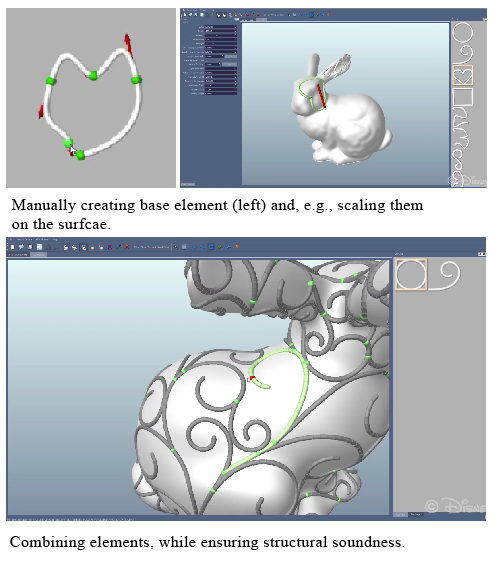
\includegraphics[width=\linewidth]{figures/discussion/zehnder_2016_dso.png}}
    \caption{\label{fig:zehnder_2016_dso}\citeauthor*{zehnder_2016_dso}~\cite{zehnder_2016_dso} offer various control mechanisms, from creating the base elements (top-left) to combining and editing them on the surface, while ensuring structural soundness (bottom). Examples are from the supplemental video.}
\end{figure}

In terms of control mechanisms for a more complex design goal, shapes and masks do not permit hierarchical or element-level local controls or the control of element connections needed by artists who want to generate patterns creatively without having to write code.


\subsection{Fields}
\label{subsubsec:analysis_creative_means_fields}

Fields (in the context of this survey, usually vector fields) constitute a powerful tool for combining automatic procedural filling with the option to direct the process in specific regions, usually with direct control on the canvas. As \citeauthor*{hsu_2020_aef}~\cite{hsu_2020_aef}, ~\citeauthor*{saputra_2017_ffo}~\cite{saputra_2017_ffo} and \citeauthor*{gieseke_2017_ooo}~\cite{gieseke_2017_ooo} show (\Cref{fig:fields}), the streamlines of a field can structure how a space is filled. Using a vector field to control, \eg directionality, can greatly decrease the manual work needed to fill a space in its entirety because a few curves can define the entire field. Other global design choices, such as an overall growth direction or the alignment of elements, are simple to translate from a vector field to procedural generation rules.

\begin{figure*}
    \centering
    \revimage{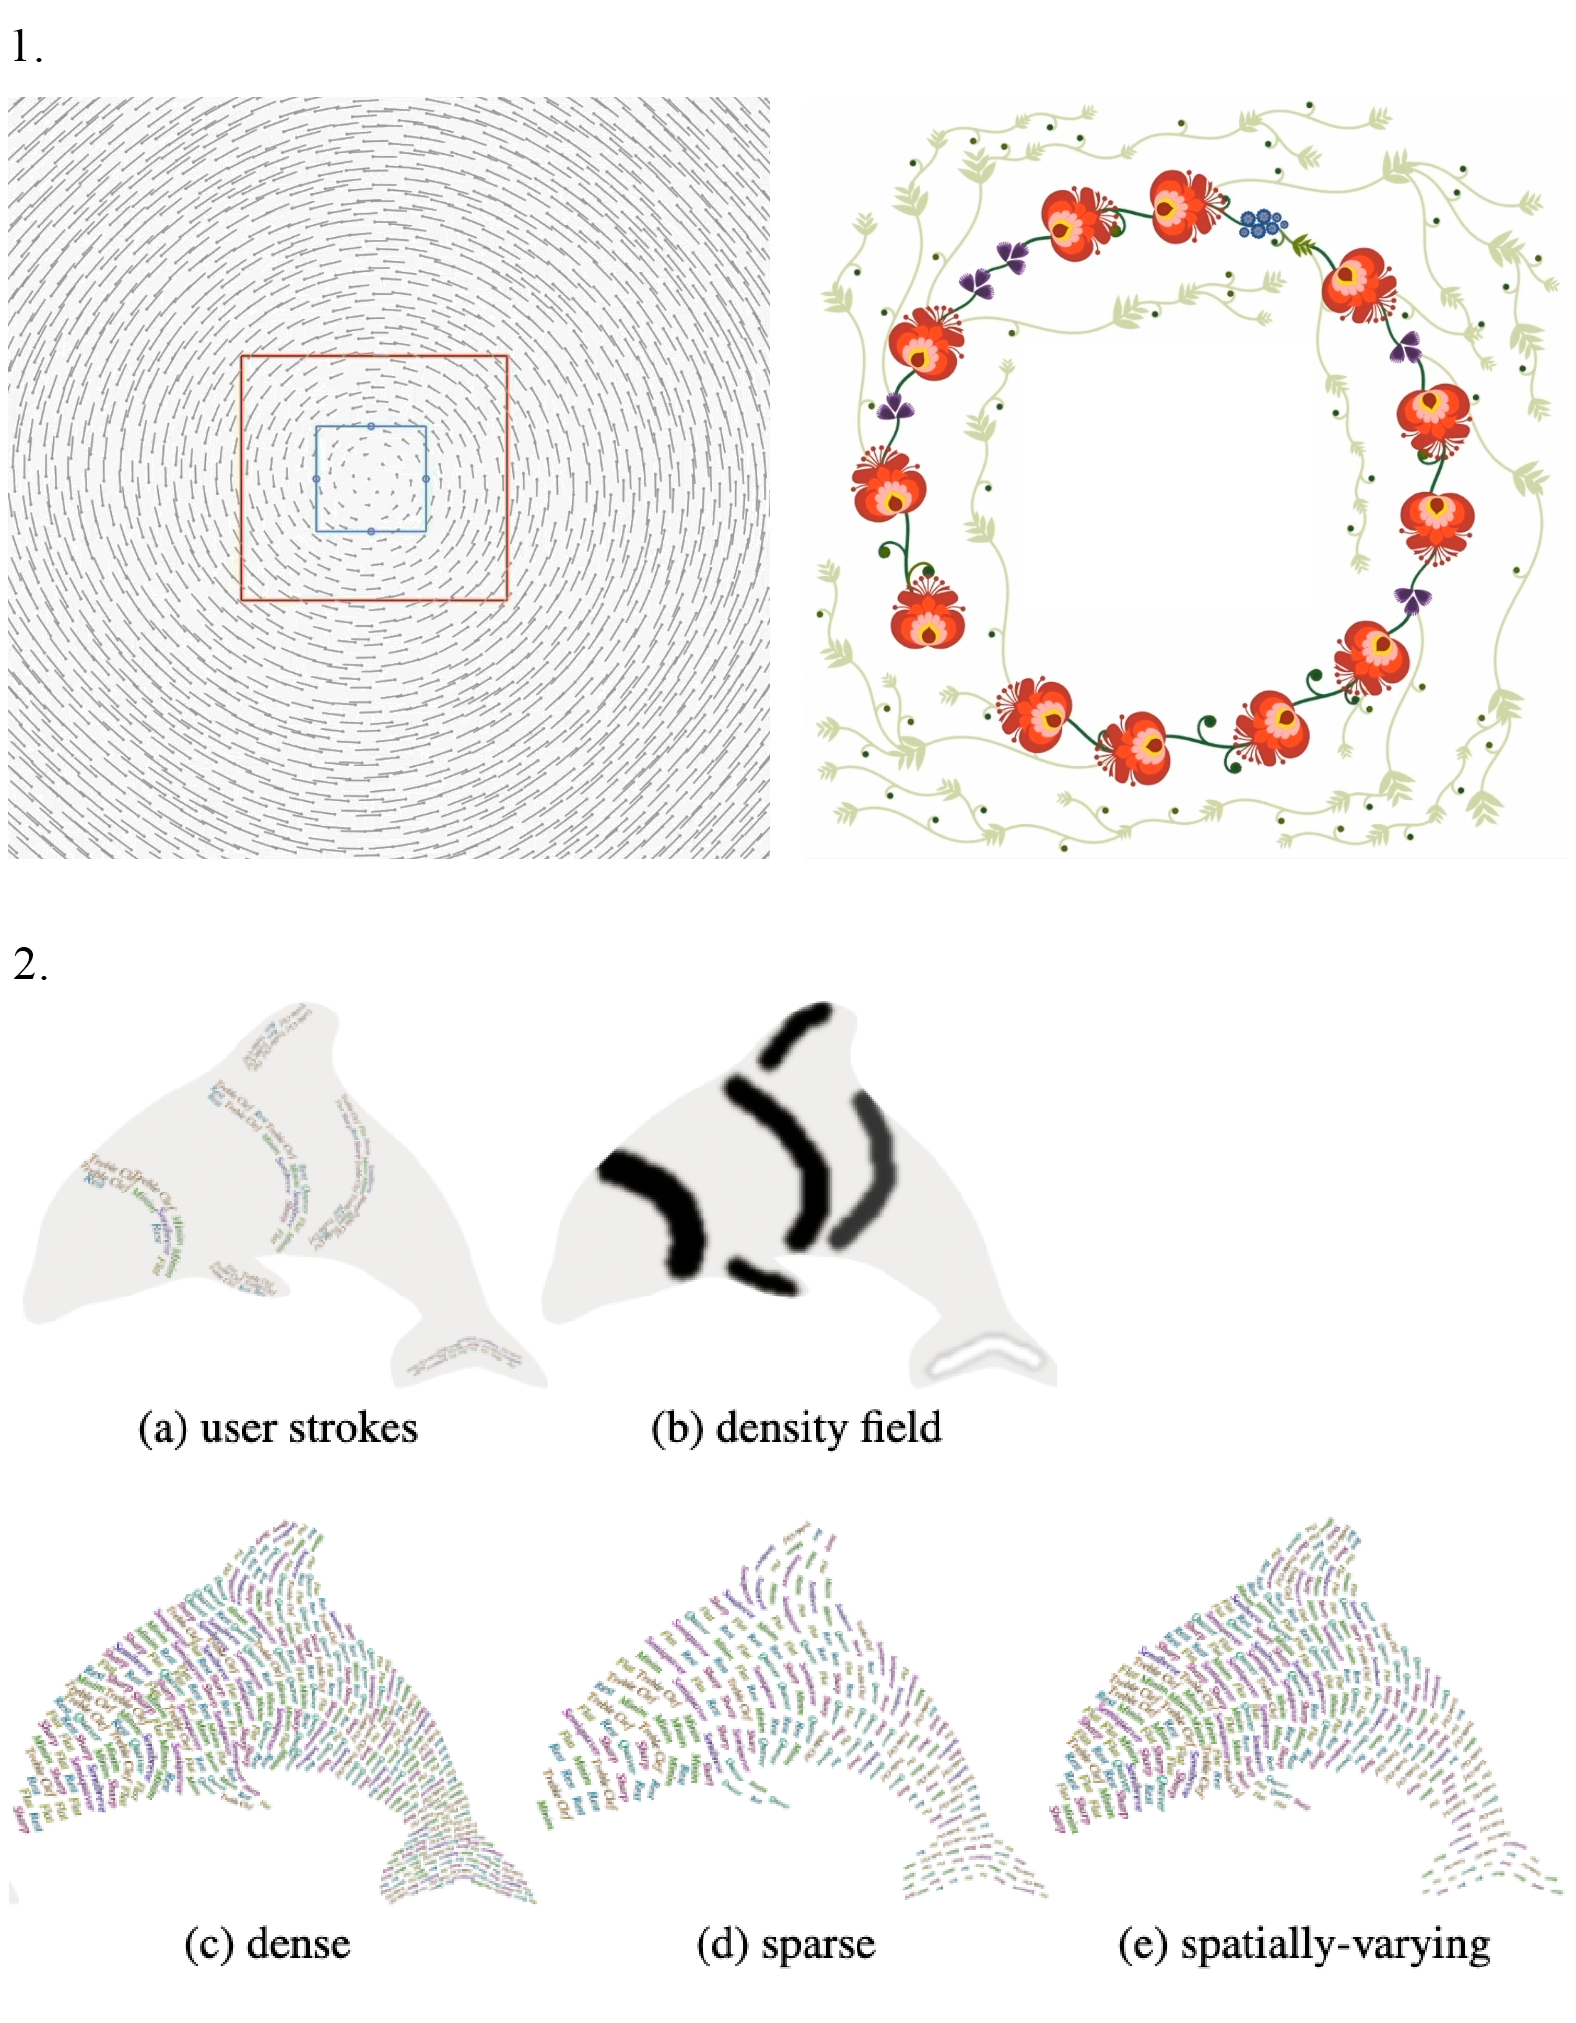
\includegraphics[width=\linewidth]{figures/discussion/fields.png}}
    \caption{\label{fig:fields}Different approaches to using vector fields for creative pattern generation. 1.~\citeauthor*{gieseke_2017_ooo}~\cite{gieseke_2017_ooo} (example from the supplemental video), 2.~\citeauthor*{hsu_2020_aef}~\cite{hsu_2020_aef}, 3.~\citeauthor*{saputra_2017_ffo}~\cite{saputra_2017_ffo}.}
\end{figure*}

The discussed work shows that fields allow for greater visual variation by opening the design space and  providing transparent control for filling a space automatically. While fields are still a level of abstraction away from the pattern itself, they are intuitive to understand, \eg through a visual representation. Their abstraction translates to the model in a straightforward manner. Thus, using flow within a vector field to design is a suitable control mechanism, especially for designs that aims to align their elements to the space.


\subsection{Curves and Brushing}
\label{subsubsec:analysis_creative_means_curves}

Curves and hand-drawn paths give an artist direct control over the final result, putting the control directly onto the canvas. Curves are needed for tasks such as creating a decorative frame or structuring a space. Some techniques consider the whole curve before computing the ornament and optimize the filling of the curve based on certain design goals. This can be understood as a form of global planning. 

\begin{figure}
    \centering
    \revimage{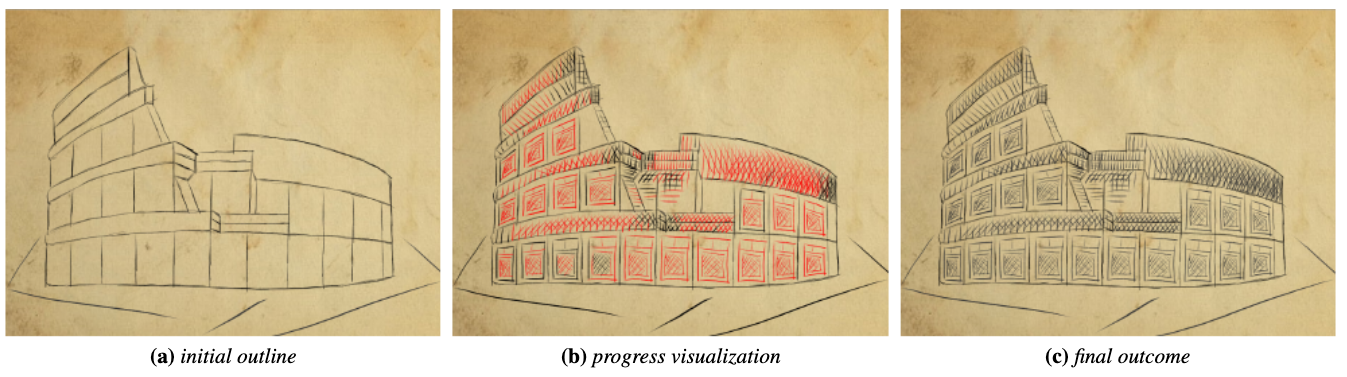
\includegraphics[width=\linewidth]{figures/discussion/xing_2014_apr.png}}
    \caption{\label{fig:xing_2014_apr}\citeauthor*{xing_2014_apr}~\cite{xing_2014_apr} propagate user sketches (right, black strokes) to fill an outline automatically (right, red strokes).}
\end{figure}

Curves and sketch-like methods offer well-communicated, transparent navigation. The discussed techniques are mostly interactive, and artists are familiar with their functionality from the real world and how they work directly on the canvas. The ease and directness of usage also constitute a foundation for possible immersive flow of work. Painting-like methods can support smoother navigation by integrating brush settings and increasing the quantity of controls. 

On the downside, curves and brushing could lead to tedious manual creation requirements for patterns and unstructured results. To balance this, \citeauthor*{kazi_2012_vit}~\cite{kazi_2012_vit} and \citeauthor*{xing_2014_apr}~\cite{xing_2014_apr} (\Cref{fig:xing_2014_apr}) incorporate procedural creation principles into a data-driven process. \citeauthor*{hsu_2020_aef}~\cite{hsu_2020_aef} offer an intuitive and transparent navigation through a brushing system, letting artists realize their design goals for element arrangements. \rev{}{The approach of~\citeauthor*{li_2020_sva}~\cite{li_2020_sva} combines visual curve creation, code, and data in a unique manner by showing textual and numeric information about the underlying procedural algorithm on the canvas. The technique might increases a transparent and navigable workflow once an artist has learned the workflow. This novel approach calls for further investigation and verification.}

% \begin{figure}[H]
%     \centering
%     \revimage{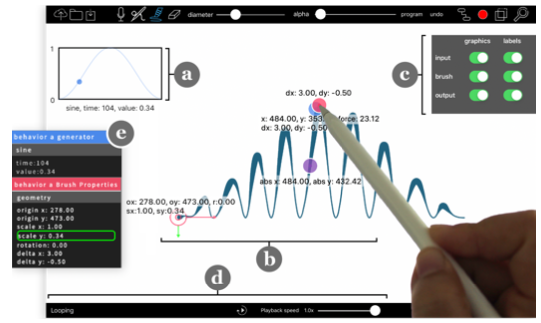
\includegraphics[width=\linewidth]{figures/discussion/li_2020_sva.png}}
%     \caption{\label{fig:li_2020_sva}\citeauthor*{li_2020_sva}~\cite{li_2020_sva}s' technique (Figure 1) links visual output, data and code with (a) visualizations, (b) iconography, (c) inspection toggles, and (d) looping controls. \color{orange}{Status rights: requested}}
% \end{figure}


In summary, brushes let artists draw almost anything, depending only on their drawing capabilities. For creative pattern generation, however, structure, pattern hierarchies, and distribution techniques also need to be supported. \revremove{}{Hence, element arrangements can only provide a subset - albeit an important one - of the design space needed for creative pattern generation.}



\subsection{Element Placement}
\label{subsubsec:analysis_creative_means_elements}

Placing single elements onto the canvas maximizes artist control and is on its own a trivial data-driven control principle. However, this mechanism becomes interesting in combination with procedural modeling. Separately placed elements that do not follow any rules should be integrated and processed to remain part of the underlying global scene structure, as demonstrated by \citeauthor*{gieseke_2017_ooo}~\cite{gieseke_2017_ooo}.
\revremove{}{Even though single element placements can be compared to using the tip of a brush, paint-like procedural modeling techniques often have a more spray-can-like quality.}
Element placement control mechanisms are closely related to data-driven sketch-based techniques and represent a promising approach for integrating procedural modeling functionalities into a data-driven process. \citeauthor*{guerrero_2016_pep}~\cite{guerrero_2016_pep} present an overall transparently navigable and stimulating control mechanism (\Cref{fig:guerrero_2016_pep}). The carefully designed workflow fosters artist stimulation by offering novel but suitable design variations.

\begin{figure}
    \centering
    \revimage{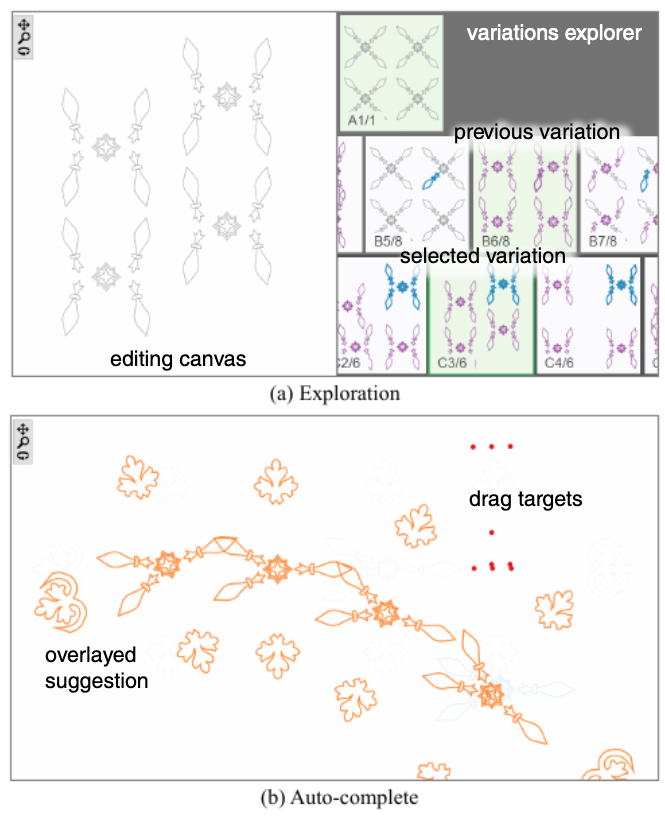
\includegraphics[width=\linewidth]{figures/discussion/guerrero_2016_pep.png}}
    \caption{\label{fig:guerrero_2016_pep}\citeauthor*{guerrero_2016_pep}~\cite{guerrero_2016_pep} combine the exploration of pattern variations with manual editing of single elements, \eg by drag and drop.}
\end{figure}